\chapter{How to Install}

\section{How This Book Makes Money}
\subsection{The Economics of Sharing Knowledge}
This book follows an innovative funding model inspired by the principles of openness and accessibility. To ensure everyone can benefit, a free version of the book is available online. However, creating a resource of this quality takes significant effort, so we provide additional options for readers who want to support this project:

\begin{itemize}
\item \textbf{Free Version}: A digital copy available for free download on the website.
\item \textbf{Textbook Version}: A polished, printed version of the book available for purchase at an affordable price.
\item \textbf{Fancy Auction Edition}: A collector\textquoteright s edition, hand-bound with unique illustrations, auctioned to the highest bidder.
\end{itemize}

\subsection{Transparency in Funding}
Here is a sample breakdown of the revenue split for the textbook version.
\begin{itemize}
\item \textbf{50}: Publishing (Vetro Editions \cite{vetro}), for actually making a book
\item \textbf{10}: Artistic Contributors (Marie), for her inspiration throughout the years
\item \textbf{20}: Institutional Contributors (Bhante G, Sayadaw U Thuzana), for their low cost and widely available monasteries, Bhavana Society \cite{bhavana} and TMC \cite{tmc}, and their charitable projects abroad.
\item \textbf{20}: Other Contributors (Geoffrey Bradway, Robert Rhyne, Brian Chamowitz, and Bhante Kheminda)

\end{itemize}

\subsection{Why It Matters}
This funding model helps bridge the gap between accessibility and sustainability. By supporting this project in any way\textemdash whether through donations, buying a book, or bidding on the fancy edition\textemdash you\textquoteright re contributing to a more inclusive knowledge-sharing ecosystem.

\section{Free as in Food: Open Source Philosophy}
\subsection{Free vs. Free: Freedom and Cost}
Open source isn\textquoteright t just about free access; it\textquoteright s about the freedom to learn, share, and modify. Think of it as a community potluck: everyone brings something to the table, and everyone eats for free.

\subsection{Why Open Source is Integral to This Book}
This book was created using open-source tools, such as:
\begin{itemize}
\item \textbf{Programming}: Python and Jupyter Notebooks.
\item \textbf{Design}: Inkscape and GIMP.
\item \textbf{Collaboration}: Git and GitHub.
\end{itemize}

\subsection{Contributing to Open Source}
Readers are encouraged to contribute by:
\begin{itemize}
\item Reporting typos or errors.
\item Sharing your experiences with the book.
\item Developing additional resources for the community.
\end{itemize}

\section{Finding the Good Store: Tools and Resources}
\subsection{Essentials}
To follow along with this book, you\textquoteright ll need the following:
\begin{itemize}
\item \textbf{A Text Editor}: Visual Studio Code or Atom.
\item \textbf{Programming Language}: Python (downloadable at \url{https://python.org}).
\item \textbf{Package Manager}: pip or conda for managing libraries.
\end{itemize}

\subsection{Quality Over Quantity}
Not all resources are created equal. Focus on trusted sources like:
\begin{itemize}
\item \textbf{Documentation}: Official Python docs or reputable tutorials.
\item \textbf{Communities}: Stack Overflow, Reddit\textquoteright s r/learnpython.
\end{itemize}

\subsection{Staying Updated}
Technology evolves rapidly. To stay up-to-date:
\begin{itemize}
\item Subscribe to newsletters like PyCoder\textquoteright s Weekly.
\item Follow contributors on GitHub.
\item Join relevant online forums.
\end{itemize}

\section{Buy Me a Coffee: Supporting Creators}
\subsection{The Power of Patronage}
Supporting creators goes beyond monetary contributions. It\textquoteright s about valuing their work and ensuring they can continue to produce.

\subsection{Ways to Support}
Here\textquoteright s how you can support this book\textquoteright s ongoing development:
\begin{itemize}
\item \textbf{Donate}: Use the \textquotedblleft Buy Me a Coffee\textquotedblright  button on the website.
\item \textbf{Purchase}: Buy the textbook version for yourself or as a gift.
\item \textbf{Promote}: Share the book with friends or leave a review.
\end{itemize}

\subsection{Paying It Forward}
If you\textquoteright ve benefited from this book, consider how you can give back, whether through mentorship, creating your own resources, or contributing to open-source projects.

\section{The CapTable}
\subsection{What\textquoteright s a CapTable?}
A cap table, short for capitalization table, is a breakdown of who owns what in a project or company. For this book, think of it as a metaphor for how value is distributed.

\subsection{Applying the CapTable to Knowledge Sharing}
In this context:
\begin{itemize}
\item \textbf{Creators}: Receive support for their work.
\item \textbf{Contributors}: Gain recognition and experience.
\item \textbf{Community}: Benefits from shared resources and tools.
\end{itemize}

\subsection{Case Studies}
Examples of successful open-source funding:
\begin{itemize}
\item Blender, funded by community-driven campaigns.
\item Wikipedia, sustained by small donations from millions of users.
\end{itemize}

\section{The Magic of Copying and Pasting}
\subsection{Efficiency in Learning}
Copy-pasting code is a great way to:
\begin{itemize}
\item Quickly test examples.
\item Explore how snippets work in practice.
\end{itemize}

\subsection{Copying Ethically}
Always:
\begin{itemize}
\item Credit the original source.
\item Understand the code before using it.
\end{itemize}

\subsection{Beyond Copy-Pasting}
Copy-pasting is just the start. Use snippets as a foundation to:
\begin{itemize}
\item Modify and experiment.
\item Develop deeper insights into programming.
\end{itemize}

\begin{figure}[h!]
    \centering
    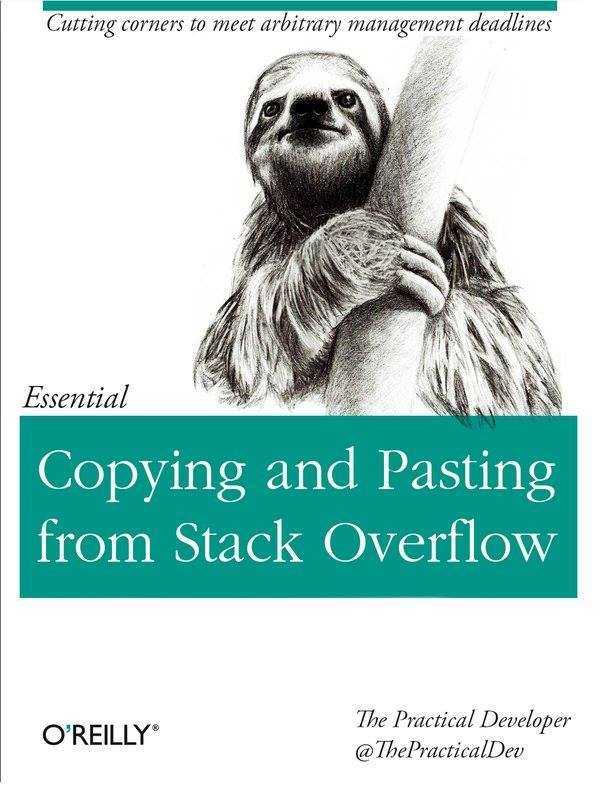
\includegraphics[width=0.8\textwidth]{figures/copypasta.jpg}
    \caption{What's this, another joke?}
    \label{fig:copypasta}
\end{figure}

\section*{Chapter Summary}
In this chapter, we explored:
\begin{itemize}
\item How this book is funded and the importance of supporting creators.
\item The philosophy of open source and its role in this project.
\item Tools and resources to get started.
\item Ethical and practical ways to engage with the content.
\end{itemize}

By understanding these principles, you\textquoteright re not just learning to install tools; you\textquoteright re joining a vibrant community of creators and learners. Welcome to the journey!
